\chapter{Implementasi dan Pengujian Perangkat Lunak}
\label{chap:Implementasi dan Pengujian Perangkat Lunak}

\section{Implementasi Perangkat Lunak}

\subsection{Lingkungan Perangkat Kerat}

Perangkat keras yang digunakan dalam membangun perangkat lunak adalah sebuah PC dengan spesifikasi berikut:

\begin{itemize}
\item \textit{Processor}: Intel i7 4790K @4.00 GHz

\item RAM: 16 GB DDR3

\item VGA: NVIDIA GeForce GTX 750TI 2GB

\item \textit{Harddisk}: 1TB + 256GB SSD 

\end{itemize}

\subsection{Lingkungan Perangkat Lunak}

Perangkat lunak yang digunakan untuk membangung perangkat lunak adalah sebagai berikut:

\begin{itemize}

\item Sistem Operasi: Ubuntu 18.04.2 LTS

\item Bahasa Pemrograman: Scala

\item IDE: InteliJ IDE 2018

\item Versi Java: JDK 1.8.0\_181

\item Versi Scala: Scala 2.11.12

\item Versi SBT: SBT 1.2.8

\item Library Dependency:

\begin{itemize}
\item org.apache.spark:spark-core 2.1.0

\item org.scala-lang:scala-library 2.11.12
\end{itemize}

\end{itemize}


\subsection{User Interface}

Implementasi rancangan tampilan antarmuka pada perangkat lunak ini menggunakan html,css, dan php. Berikut adalah tampilan setiap halaman:

\begin{enumerate}
\item Implementasi antarmuka untuk menu \textit{Submit} dapat dilihat pada Gambar ~\ref{fig:menusubmit}.

\begin{figure}[H]
    \centering  
    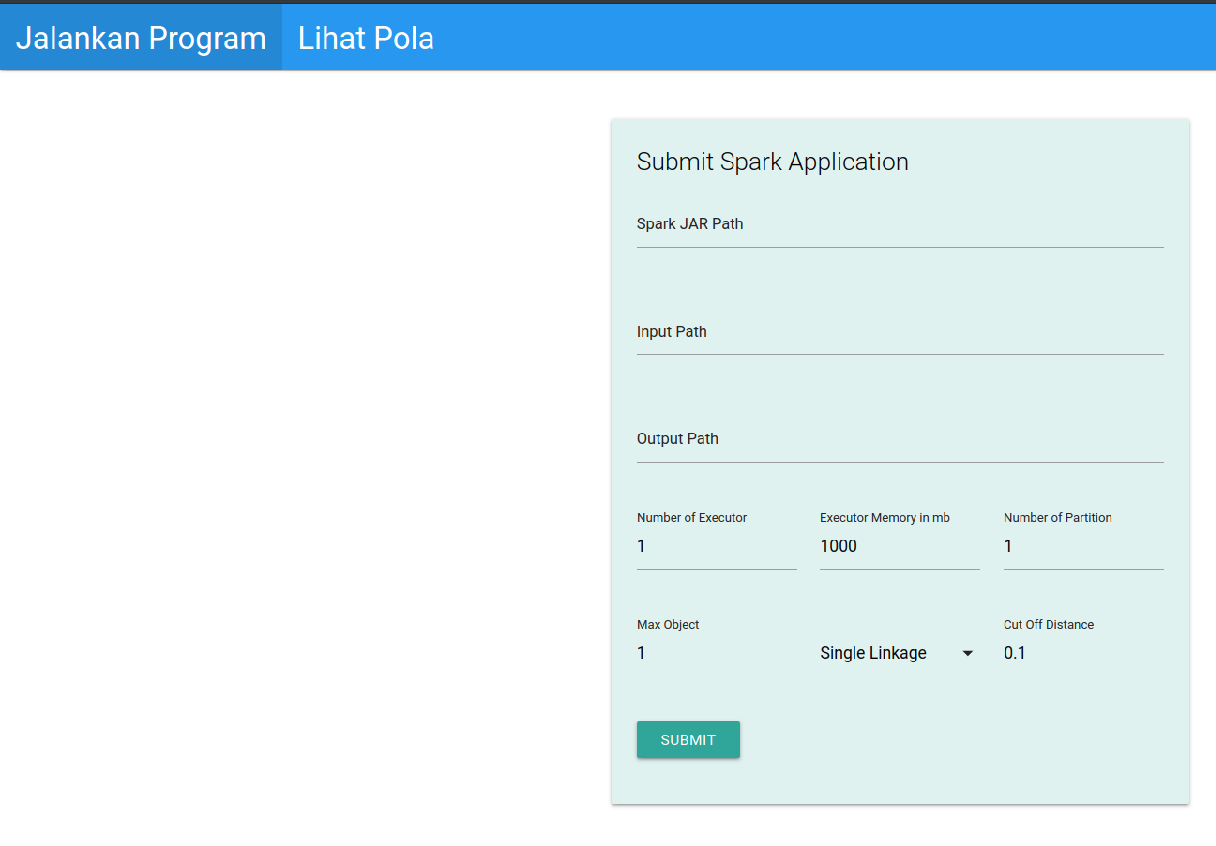
\includegraphics[scale=0.3]{menusubmit}  
    \caption[Tampilan menu \textit{Submit}]{Tampilan menu \textit{submit}} 
    \label{fig:menusubmit} 
\end{figure}

\item Implementasi antarmuka untuk menu \textit{Data} dapat dilihat pada Gambar ~\ref{fig:menudata}.

\begin{figure}[H]
    \centering  
    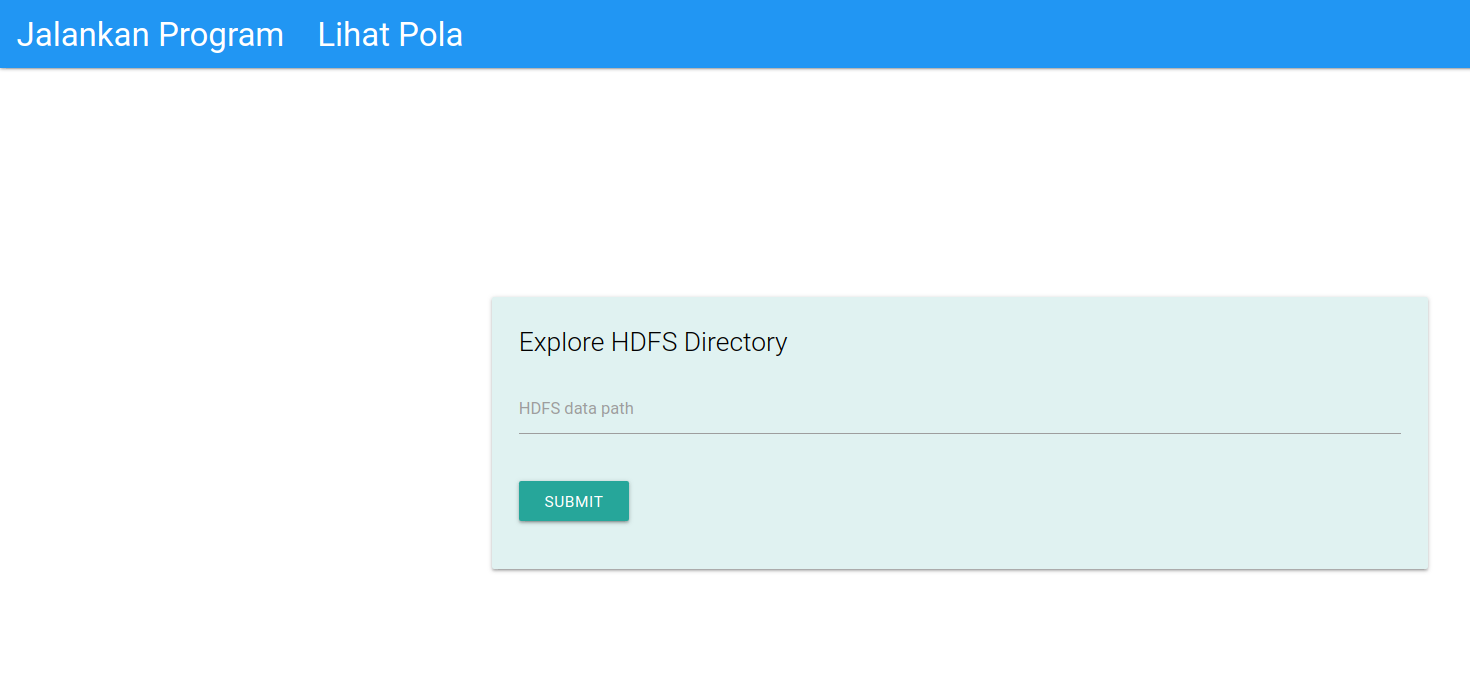
\includegraphics[scale=0.3]{menudata}  
    \caption[Tampilan menu \textit{Data}]{Tampilan menu \textit{Data}} 
    \label{fig:menudata} 
\end{figure}

\item Implementasi antarmuka sesudah melakukan \textit{submit} dapat dilihat pada Gambar ~\ref{fig:menuresult}.

\begin{figure}[H]
    \centering  
    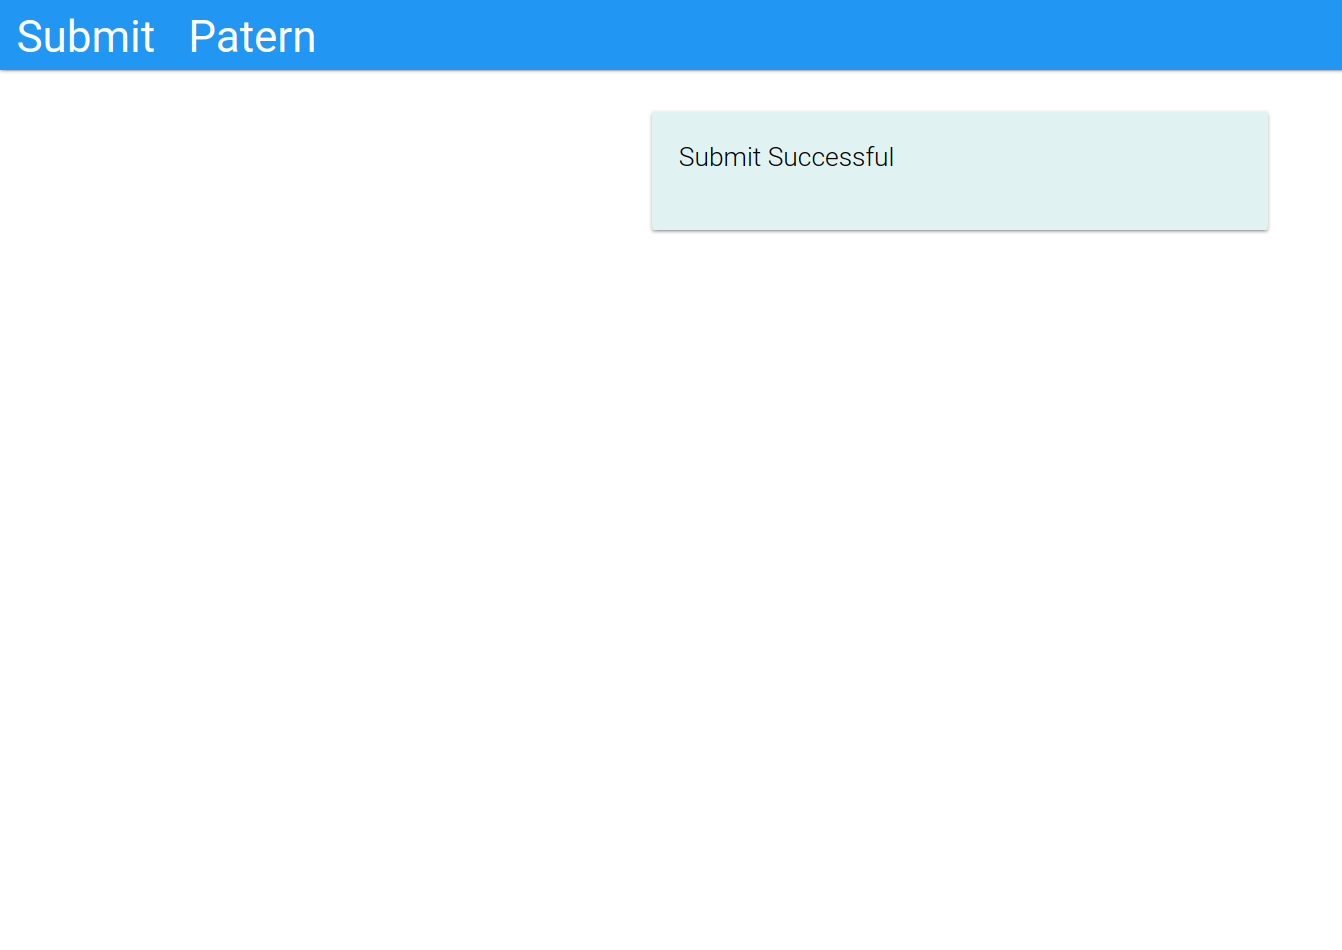
\includegraphics[scale=0.3]{menuresult}  
    \caption[Tampilan halaman sesudah \textit{submit}]{Tampilan halaman sesudah \textit{submit}} 
    \label{fig:menuresult} 
\end{figure}

\item Implementasi antarmuka  halaman \textit{list} dapat dilihat pada Gambar ~\ref{fig:menulist}.

\begin{figure}[H]
    \centering  
    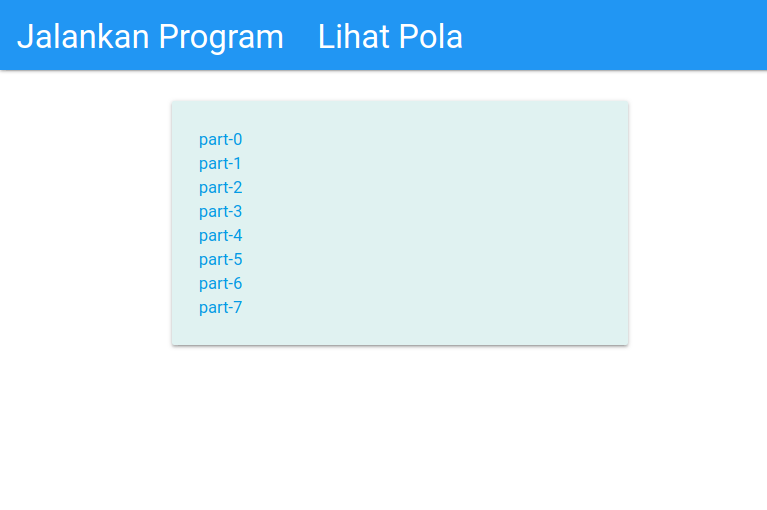
\includegraphics[scale=0.5]{menulist}  
    \caption[Tampilan halaman \textit{list}]{Tampilan halaman \textit{list}} 
    \label{fig:menulist} 
\end{figure}

\item Implementasi antarmuka  halaman \textit{data} dapat dilihat pada Gambar ~\ref{fig:menudata2}.

\begin{figure}[H]
    \centering  
    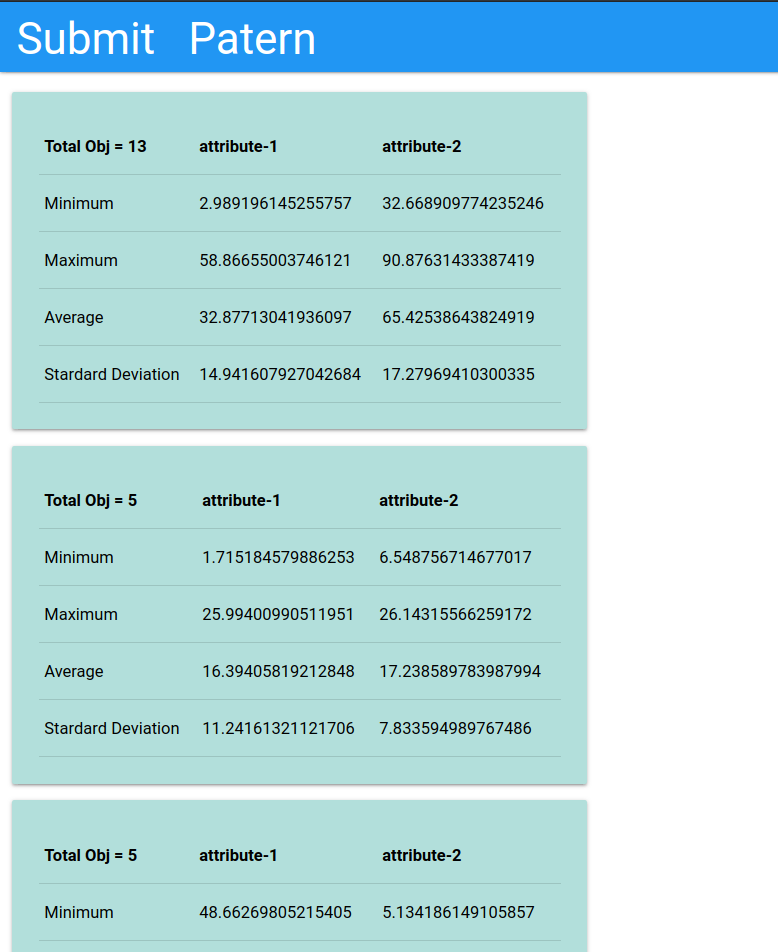
\includegraphics[scale=0.5]{menudata2}  
    \caption[Tampilan halaman data]{Tampilan halaman data} 
    \label{fig:menudata2} 
\end{figure}

\end{enumerate}

\section{Pengujian Perangkat Lunak}

Perangkat lunak yang disusun oleh penulis telah diuji untuk membuktikan kebenaran dari perangkat lunak. Program akan dieksekusi dan kemudian diamati apakah hasil sesuai dengan yang diinginkan. Perangkat lunak akan diberikan data dengan ukuran yang kecil berserta \textit{parameter} yang sudah ditentukan. 

\begin{itemize}

\item Pada percobaan pertama, akan digunakan metode \textit{single linkage}, dengan jumlah partisi = 1, jumlah objek maksimum = 4, dan nilai \textit{cut-off distance} = 0.8. Berikut adalah data yang digunakan untuk pengujian:

\begin{verbatim}
4.0,5.0
3.0,7.0
4.0,3.0
10.0,7.0
10.0,10.0
\end{verbatim}

Hasil dari percobaan pertama adalah sebagai berikut:

\begin{verbatim}
3
3.0,3.0
4.0,7.0
3.6666666666666665,5.0
0.5773502691896258,2.0
1
10.0,7.0
10.0,7.0
10.0,7.0
0.0,0.0
1
10.0,10.0
10.0,10.0
10.0,10.0
0.0,0.0
\end{verbatim}

\item Pada percobaan kedua, akan digunakan metode \textit{complete linkage}, dengan jumlah partisi = 1, jumlah objek maksimum = 4, dan nilai \textit{cut-off distance} = 0.8. Berikut adalah data yang digunakan untuk pengujian:

\begin{verbatim}
4.0,5.0
3.0,7.0
4.0,3.0
10.0,7.0
10.0,10.0
\end{verbatim}

Hasil dari percobaan kedua adalah sebagai berikut:

\begin{verbatim}
3
3.0,3.0
4.0,7.0
3.6666666666666665,5.0
0.5773502691896258,2.0
1
10.0,7.0
10.0,7.0
10.0,7.0
0.0,0.0
1
10.0,10.0
10.0,10.0
10.0,10.0
0.0,0.0
\end{verbatim}

\item Pada percobaan ketiga, akan digunakan metode \textit{centroid linkage}, dengan jumlah partisi = 1, jumlah objek maksimum = 4, dan nilai \textit{cut-off distance} = 0.8. Berikut adalah data yang digunakan untuk pengujian:

\begin{verbatim}
4.0,5.0
3.0,7.0
4.0,3.0
10.0,7.0
10.0,10.0
\end{verbatim}

Hasil dari percobaan ketiga adalah sebagai berikut:

\begin{verbatim}
3
3.0,3.0
4.0,7.0
3.6666666666666665,5.0
0.5773502691896258,2.0
1
10.0,7.0
10.0,7.0
10.0,7.0
0.0,0.0
1
10.0,10.0
10.0,10.0
10.0,10.0
0.0,0.0
\end{verbatim}

 
\end{itemize}

Berdasarkan hasil ketiga percobaan yang didapat, maka dapat disimpulkan bahwa perangkat lunak sudah dapat melakukan proses reduksi data menggunakan algoritma \textit{Agglomerative Clustering} berdasarkan metode yang dipilih dengan benar. Pola yang dihasilkan oleh perangkat lunak sudah sesuai dengan apa yang diharapakan.

\section{Perbandingan Performa Perangkat Lunak}

Pada bagian ini akan diuji performa perangkat lunak Spark dan Hadoop. Kedua perangkat lunak akan dibandingkan hasil eksekusi waktunya. Karena perangkat lunak hadoop tidak dapat menghitung standard deviasi, maka perangkat lunak Hadoop akan dibandingkan dengan perangkat lunak Spark yang tidak menghitung standard deviasi dan yang menghitung standard deviasi. Data yang digunakan pada percobaan merupakan data yang dihasilkan secara acak dengan ukuran yang berbeda-beda. Data-data tersebut memiliki dua atribut bilangan pecahan yang dipisahkan dengan tanda koma. Jumlah objek pada setiap ukuran data dapat dilihat pada Tabel ~\ref{tab:exdata}.\\

\begin{table}[H] 
	\centering 
	\caption{Tabel data yang digunakan pada eksperimen}
	\label{tab:exdata}
	\begin{tabular}{|p{2cm}|p{4cm}|}
\hline
Ukuran Data & Jumlah Objek  \\
\hline
20 MB & 640000 \\
\hline
30 MB & 810000 \\
\hline
40 MB & 1000000 \\
\hline
1 GB & 36000000 \\
\hline
2 GB & 64000000 \\
\hline
3 GB & 81000000 \\
\hline
5 GB & 144000000 \\
\hline
10 GB & 256000000 \\
\hline
15 GB & 400000000 \\
\hline
20 GB & 529000000 \\
\hline
	\end{tabular} 
\end{table}



Berikut adalah spesifikasi perangkat keras yang digunakan:

\begin{itemize}

\item \textit{Processor}: Intel core i5 8500 @3.00 GHz, 6 \textit{core}

\item RAM: 8GB

\item \textit{Harddisk}: 500GB

\item Sistem Operasi: Ubuntu 18.0.4

\end{itemize}


Pada percobaan pertama akan digunakan 1 komputer sebagai komputer \textit{master} dan 10 komputer sebagai \textit{worker} untuk memproses data-data yang berukuran berbeda. Setiap worker menggunakan 1 core. Metode yang digunakan adalah metode \textit{single-linkage}, dengan nilai \textit{cut-off distance} 0.8, dengan jumlah objek maksimum adalah 30, dan jumlah partisi adalah 10. UKuran block yang digunakan pada HDFS adalah 32MB. Tabel (~\ref{tab:spark10}) berikut adalah hasil dari eksperimen:

\begin{table}[H] 
	\centering 
	\caption{Tabel hasil percobaan perbandingan Hadoop dan Spark}
	\label{tab:spark10}
	\begin{tabular}{|p{1.5cm}|p{1cm}|p{4cm}|p{4cm}|p{3cm}|}
\hline
Ukuran Data & Jumlah Partisi & Waktu Ekseuksi Spark (tanpa standard deviasi) & Waktu Eksekusi Spark & Waktu Eksekusi Hadoop  \\
\hline
1 GB & 10 & 113 detik & 118 detik & 183 detik\\
\hline
2 GB & 10 & 165 detik & 195 detik & 252 detik\\
\hline
3 GB & 10 & 209 detik & 214 detik & 318 detik\\
\hline
5 GB & 10 & 327 detik & 343 detik & 505 detik\\
\hline
10 GB & 10 & 570 detik & 578 detik & 953 detik\\
\hline
15 GB & 10 & 863 detik & 874 detik & 1434 detik\\
\hline
20 GB & 10 & 1131 detik & 1111 detik & 1830 detik\\
\hline

\hline
	\end{tabular} 
\end{table}

\def\scl{1}
% \def\leg{\legend{Switching,Homotopic,Buffer*Length,Length}}
\def\leg{} 
\def\std{none}
\def\ymin{}
\def\ymax{}

\begin{minipage}[c]{0.9\textwidth}
	\begin{figure}[H]
		\centering
		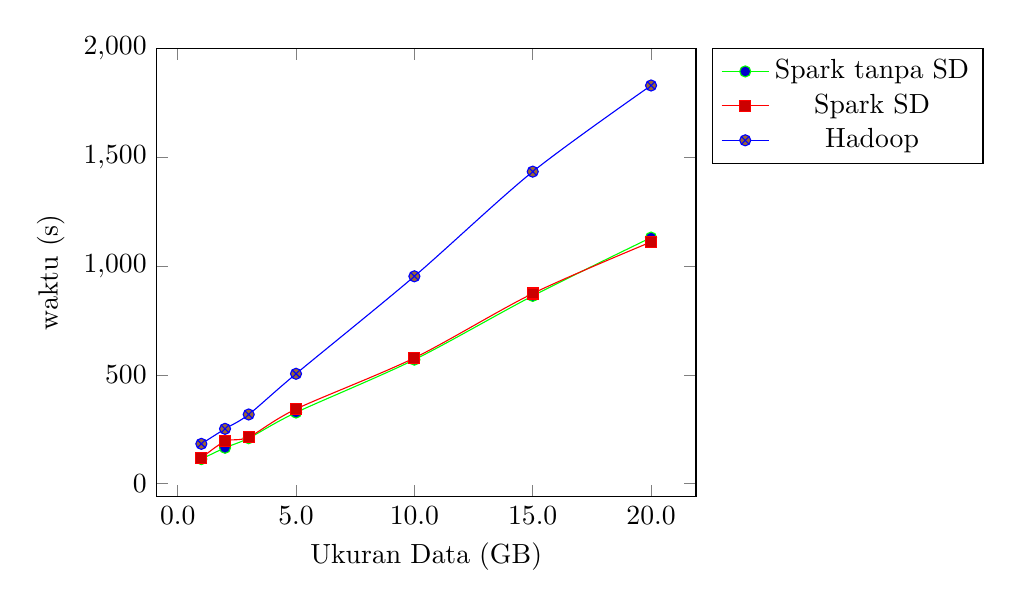
\begin{tikzpicture}[scale=\scl]
		\begin{axis}[\ymin,\ymax,xlabel= Ukuran Data (GB),ylabel= waktu (s), xticklabel style={/pgf/number format/.cd, fixed,fixed zerofill, precision=1},legend pos = outer north east]
		
		\addlegendentry{Spark tanpa SD}
		\addplot+[smooth][color=green] coordinates {(1,113) (2,165) (3,209) (5,327) (10,570) (15,863) (20,1131)};
		\addlegendentry{Spark SD}
		\addplot+[smooth][color=red] coordinates {(1,118) (2,195) (3,214) (5,343) (10,578) (15,874) (20,1111) };
		\addlegendentry{Hadoop}
		\addplot+[smooth][color=blue] coordinates {(1,183) (2,252) (3,318) (5,505) (10,953) (15,1434) (20,1830)};

		\leg
		\end{axis}
		\end{tikzpicture}
		\caption[Hasil percobaan pertama]{Hasil percobaan pertama}
		\label{fig:percobaan1}
	\end{figure}
\end{minipage}\\






Pada percobaan kedua akan digunakan 1 komputer sebagai komputer \textit{master} dan 10 komputer sebagai \textit{worker} untuk memproses data-data yang berukuran berbeda. Setiap worker menggunakan 3 core. Metode yang digunakan adalah metode \textit{single-linkage}, dengan nilai \textit{cut-off distance} 0.8, dengan jumlah objek maksimum adalah 30, dan jumlah partisi adalah 30. UKuran block yang digunakan pada HDFS adalah 32MB. Tabel (~\ref{tab:spark10}) berikut adalah hasil dari eksperimen:

\begin{table}[H] 
	\centering 
	\caption{Tabel hasil percobaan perbandingan Hadoop dan Spark}
	\label{tab:spark10}
	\begin{tabular}{|p{1.5cm}|p{1cm}|p{4cm}|p{4cm}|p{3cm}|}
\hline
Ukuran Data & Jumlah Partisi & Waktu Ekseuksi Spark (tanpa standard deviasi) & Waktu Eksekusi Spark & Waktu Eksekusi Hadoop  \\
\hline
1 GB & 30 & 83 detik & 77 detik & 85 detik\\
\hline
2 GB & 30 & 109 detik & 118 detik & 135 detik\\
\hline
3 GB & 30 & 123 detik & 150 detik & 162 detik\\
\hline
5 GB & 30 & 199 detik & 218 detik & 257 detik\\
\hline
10 GB & 30 & 327 detik & 332 detik & 459 detik\\
\hline
15 GB & 30 & 485 detik & 501 detik & 671 detik\\
\hline
20 GB & 30 & 623 detik & 677 detik & 867 detik\\
\hline

\hline
	\end{tabular} 
\end{table}

\def\scl{1}
% \def\leg{\legend{Switching,Homotopic,Buffer*Length,Length}}
\def\leg{} 
\def\std{none}
\def\ymin{}
\def\ymax{}

\begin{minipage}[c]{0.9\textwidth}
	\begin{figure}[H]
		\centering
		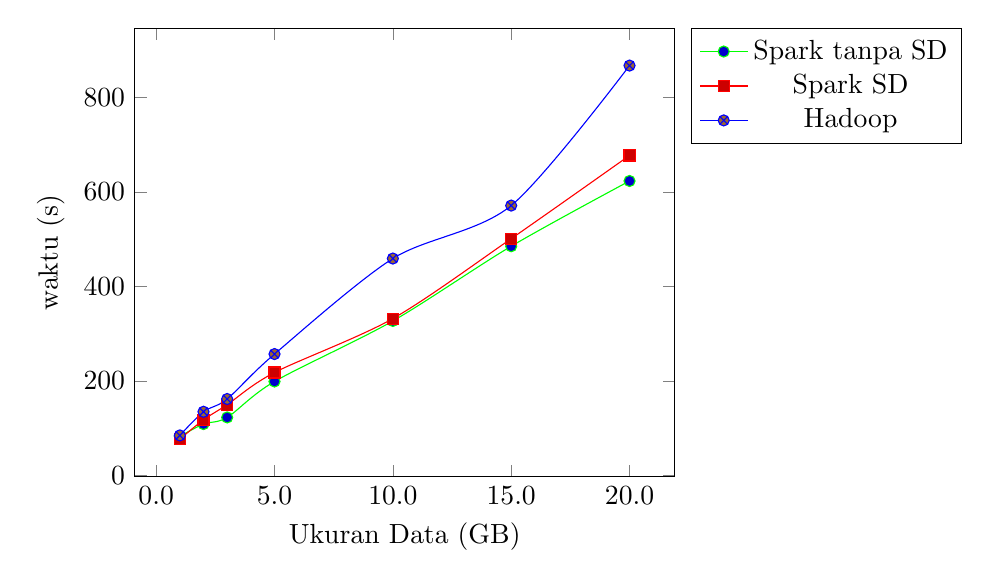
\begin{tikzpicture}[scale=\scl]
		\begin{axis}[\ymin,\ymax,xlabel= Ukuran Data (GB),ylabel= waktu (s), xticklabel style={/pgf/number format/.cd, fixed,fixed zerofill, precision=1},legend pos = outer north east]
		
		\addlegendentry{Spark tanpa SD}
		\addplot+[smooth][color=green] coordinates {(1,83) (2,109) (3,123) (5,199) (10,327) (15,485) (20,623)};
		\addlegendentry{Spark SD}
		\addplot+[smooth][color=red] coordinates {(1,77) (2,118) (3,150) (5,218) (10,332) (15,501) (20,677) };
		\addlegendentry{Hadoop}
		\addplot+[smooth][color=blue] coordinates {(1,85) (2,135) (3,162) (5,257) (10,459) (15,571) (20,867)};

		\leg
		\end{axis}
		\end{tikzpicture}
		\caption[Hasil percobaan kedua]{Hasil percobaan kedua}
		\label{fig:percobaan2}
	\end{figure}
\end{minipage}\\







Pada percobaan ketiga akan digunakan 1 komputer sebagai komputer \textit{master} dan 10 komputer sebagai \textit{worker} untuk memproses data-data yang berukuran berbeda. Setiap worker menggunakan 5 core. Metode yang digunakan adalah metode \textit{single-linkage}, dengan nilai \textit{cut-off distance} 0.8, dengan jumlah objek maksimum adalah 30, dan jumlah partisi adalah 30. UKuran block yang digunakan pada HDFS adalah 32MB. Tabel (~\ref{tab:spark10}) berikut adalah hasil dari eksperimen:

\begin{table}[H] 
	\centering 
	\caption{Tabel hasil percobaan perbandingan Hadoop dan Spark}
	\label{tab:spark10}
	\begin{tabular}{|p{1.5cm}|p{1cm}|p{4cm}|p{4cm}|p{3cm}|}
\hline
Ukuran Data & Jumlah Partisi & Waktu Ekseuksi Spark (tanpa standard deviasi) & Waktu Eksekusi Spark & Waktu Eksekusi Hadoop  \\
\hline
1 GB & 50 & 59 detik & 62 detik & 96 detik\\
\hline
2 GB & 50 & 114 detik & 116 detik & 156 detik\\
\hline
3 GB & 50 & 126 detik & 140 detik & 177 detik\\
\hline
5 GB & 50 & 220 detik & 216 detik & 294 detik\\
\hline
10 GB & 50 & 336 detik & 345 detik & 490 detik\\
\hline
15 GB & 50 & 491 detik & 534 detik & 732 detik\\
\hline
20 GB & 50 & 651 detik & 670 detik & 976 detik\\
\hline

\hline
	\end{tabular} 
\end{table}

\def\scl{1}
% \def\leg{\legend{Switching,Homotopic,Buffer*Length,Length}}
\def\leg{} 
\def\std{none}
\def\ymin{}
\def\ymax{}

\begin{minipage}[c]{0.9\textwidth}
	\begin{figure}[H]
		\centering
		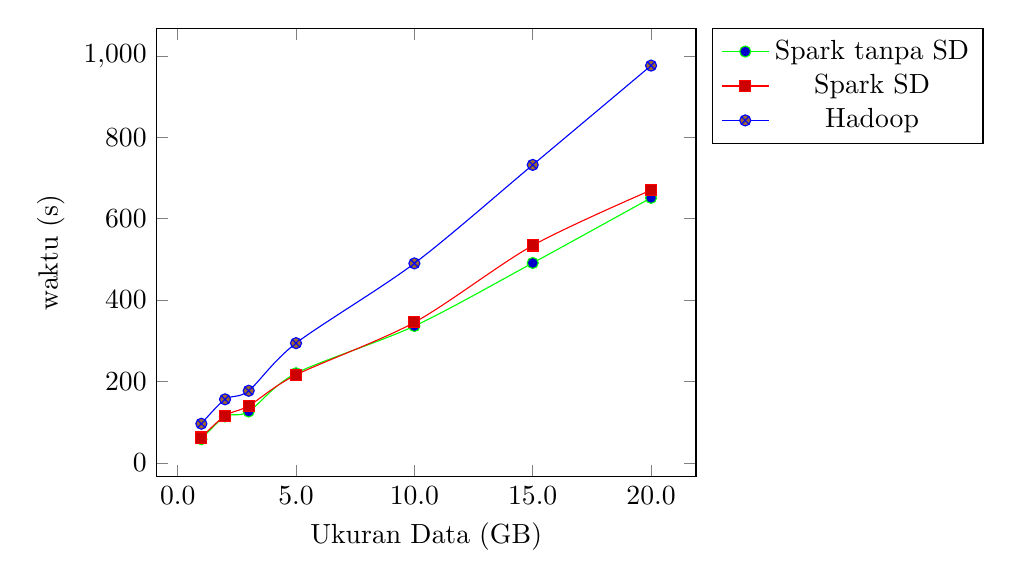
\begin{tikzpicture}[scale=\scl]
		\begin{axis}[\ymin,\ymax,xlabel= Ukuran Data (GB),ylabel= waktu (s), xticklabel style={/pgf/number format/.cd, fixed,fixed zerofill, precision=1},legend pos = outer north east]
		
		\addlegendentry{Spark tanpa SD}
		\addplot+[smooth][color=green] coordinates {(1,58) (2,114) (3,126) (5,220) (10,336) (15,491) (20,651)};
		\addlegendentry{Spark SD}
		\addplot+[smooth][color=red] coordinates {(1,62) (2,116) (3,140) (5,216) (10,345) (15,534) (20,670) };
		\addlegendentry{Hadoop}
		\addplot+[smooth][color=blue] coordinates {(1,96) (2,156) (3,177) (5,294) (10,490) (15,732) (20,976)};

		\leg
		\end{axis}
		\end{tikzpicture}
		\caption[Hasil percobaan kedua]{Hasil percobaan kedua}
		\label{fig:percobaan2}
	\end{figure}
\end{minipage}\\








